\section{Introduction}
We will talk about the data set utilized for the thesis work and its performance for various models in this part. This chapter will also cover the end results and their analysis. 
The primary objective of this research is to develop and evaluate an efficient DeepLabV3+ model with different DCNNs as backbone and ensemble them by weighted average method for the task of water bodies segmentation. The dataset used in this study annotated with ground truth masks indicating the presence of water. The research involves preprocessing the data, training the model, and fine-tuning its parameters to achieve optimal performance. Key performance metrics, such as accuracy, precision, recall, F1 score and intersection over union (IoU) are used to evaluate the model's effectiveness.The significance of this thesis is finally examined, and the assessment of this research project is concluded.

\section{Dataset Description}
For our thesis work, we have collected the remote sensing images and their corresponding masks from kaggle \cite{data1} \cite{data2} which includes a total of 2900 images.The datasets contains of two classes,which are water bodies areas, and non-water bodies areas.The dataset utilized in this thesis comprises aerial and satellite images. It is curated to provide a diverse representation of various geographic locations, ensuring the robustness and generalizability of the model. The dataset includes both synthetic and real-world images, with annotations indicating the presence and extent of water.Images are resized to a uniform dimension (e.g. 256x256 pixels) to ensure compatibility with the input requirements of the DeepLabV3+ model.Techniques such as rotation, flipping, and scaling are applied to increase the diversity of the training set and improve the model's generalizability.we divided the dataset into
80\% of dataset used to train the model, Comprises 10\% of the total dataset, used for hyperparameter tuning and model validation during training and Comprises 10\% of the total dataset, used for evaluating the final model's performance on unseen data. After that we increased
the dataset using different augmentation techniques.

\section{Experimental Setup}
We trained our all model in Kaggle that provided 16GB RAM and two 18GB T4 GPUs. We resized
our image into 256 x 256 pixels image for training our all model and used data augmentation for better performance.

\section{Evaluation of Performance}
\subsection{Evaluation Metrics}
The evaluation metrics are crucial for assessing the performance and accuracy for our model.In order to evaluate our models performance, many assessment measures are
employed. These measurements show how one model performs better than another. For our model evaluation, we settled on some metrics: Accuracy, Intersection over Union, Precision, Recall, Loss-function,F1 Score. Four words are presented from the confusion
matrix concept: True Negative (TN), True Positive (TP), False Negative (FN),
and False Positive (FP). Below is a description of them : \\ 

\begin{itemize}
    \item \textbf{True Positive: }Positive labels that are correctly classified.
    \item \textbf{True Negative: }Negative labels that are correctly classified.
    \item \textbf{False Positive: }Actual negative labels that are incorrectly predicted to be positive.
    \item \textbf{False Negative: }Actual positive labels incorrectly predicted to be negative. Our evaluation metrics are described below by equations based on TP,TN,FP and FN.
\end{itemize}

Below are the description for all the evaluation metrics that we have used for the measurement of our proposed model.

\begin{itemize}
    \item \textbf{Accuracy: }Accuracy is a common evaluation metric that measures the proportion of correctly predicted instances out of the total instances in a
dataset. It provides an overall measure of how well the model predicts the
correct class labels. \\
\begin{equation}
\text{Accuracy} = \frac{TP + TN}{TP + TN + FP + FN}
\\
\end{equation}

\item \textbf{Precision: }Precision is a metric that quantifies the proportion of correctly
predicted positive instances out of the total instances predicted as positive.
It focuses on the correctness of positive predictions, indicating how well the
model avoids false positives.
\\
\begin{equation}
\text{Precision} = \frac{TP}{TP + FP}
\end{equation}

\item \textbf{Recall: }Recall, also known as sensitivity or true positive rate, measures the
proportion of correctly predicted positive instances out of the actual positive
instances in the dataset. It highlights the model’s ability to identify true
positives and avoid false negatives.

\begin{equation}
\text{Recall} = \frac{TP}{TP + FN}
\end{equation}

\item \textbf{F1-Score: }The F1 score is a statistical measure used to evaluate the performance of a classification model. It is the harmonic mean of precision and recall, providing a single metric that balances both the model's accuracy in identifying true positives and its ability to minimize false positives and false negatives.It ranges from 0 to 1, where 1 indicates perfect precision and recall, and 0 indicates the worst performance. It is particularly useful in situations where you need to balance the trade-off between precision and recall, rather than optimizing for just one.

\begin{equation}
\text{F1-Score} = 2 \cdot \frac{\text{Precision} \cdot \text{Recall}}{\text{Precision} + \text{Recall}}
\end{equation}

\item \textbf{Loss Function: }A loss function calculates the discrepancy between predicted and actual values during model training. It quantifies the error
made by the model and guides the optimization process to minimize this
error. Different loss functions are used depending on the task, such as mean
squared error for regression or cross-entropy for classification.
\\

\item \textbf{Intersection over Union: }Intersection over Union (IoU) is an evaluation metric used to measure the accuracy of an object detector on a particular dataset. It is commonly used in segmentation tasks to compare the similarity between the predicted segmentation mask and the ground truth mask.

\begin{equation}
\text{IoU} = \frac{TP}{TP + FP + FN}
\end{equation}

The following figure \ref{iou} shows the overview of the Intersection over Union concept,which is very important for the segmentation task.

\begin{figure}[H]
    \centering
    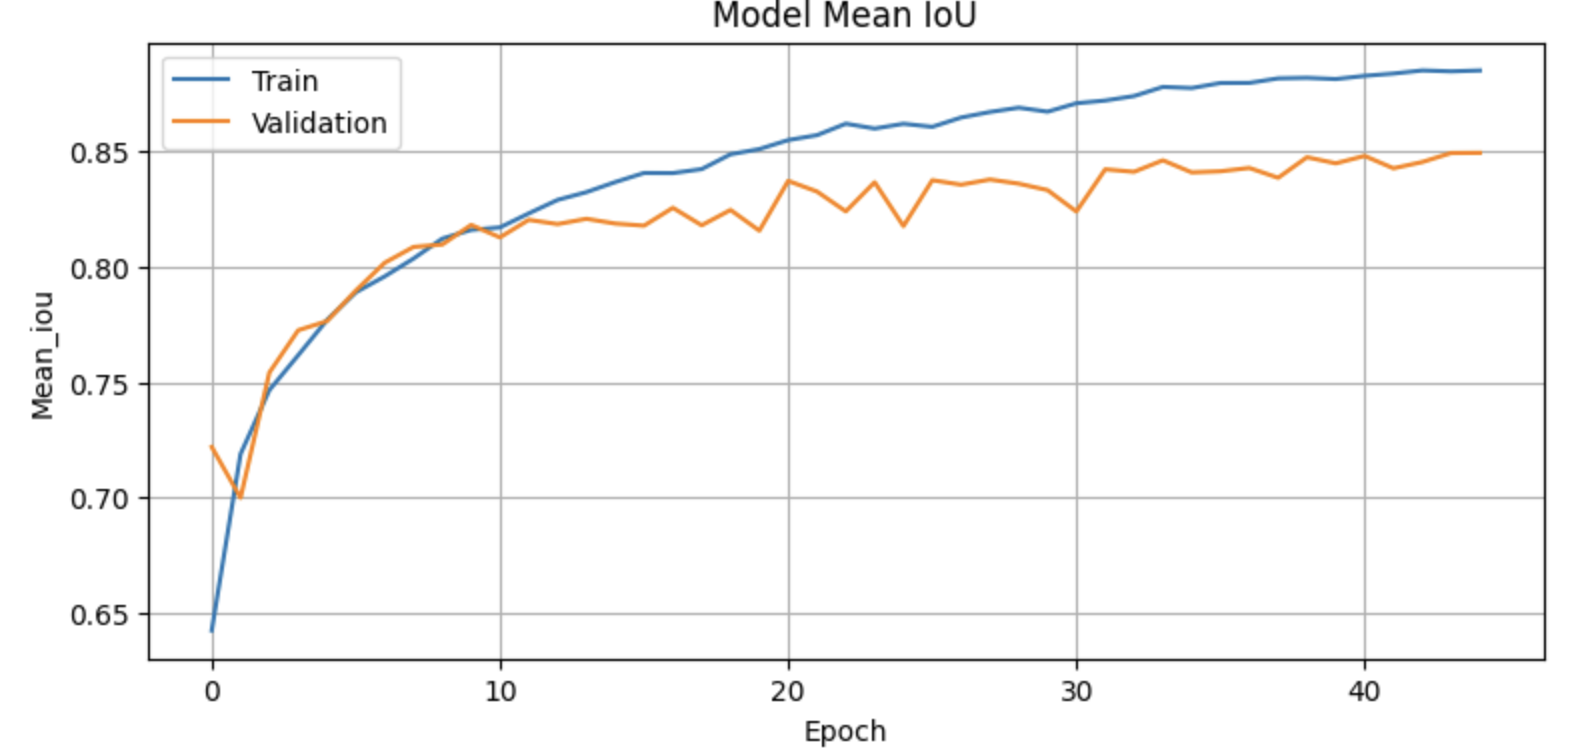
\includegraphics[width=0.8\textwidth]{figs/iou.png}
    \caption{Graphical representation of IoU}
    \label{iou}
\end{figure}

Where:
\begin{itemize}
    \item A is the set of predicted positive pixels (the predicted segmentation mask).
    \item B is the set of actual positive pixels (the ground truth segmentation mask).
    \item ∣A∩B∣ is the number of pixels where both the predicted and ground truth masks are positive (the intersection).
    \item A∪B∣ is the number of pixels where either the predicted or ground truth masks are positive (the union).
\end{itemize}
\\
IoU ranges from 0 to 1, where:
\begin{itemize}
    \item An IoU of 1 indicates perfect overlap between the predicted and ground truth masks.
    \item An IoU of 0 indicates no overlap between the predicted and ground truth masks.
\end{itemize}






\end{itemize}
\subsection{Comparison of different pre-trained model}
Comparing different pre-trained models for water bodies segmentation can provide valuable insights into their performance, robustness, and suitability for our specific application.
The different pre-trained DCNNs were tried such as VGG-19, ResNet50V2, DenseNet, MobileNetV2, EfficientNetV2 etc. The results are demonstrated in the following table:
\\


\begin{table}[htbp]
\centering
\captionsetup{font=small} % Set font size for caption
\caption{Different Pre-trained Models as Backbone for Water bodies Segmentation}
\label{tab:pretrained-models}
\normalsize % Set font size for table
\begin{tabular}{|p{2cm}|p{2.5cm}|p{2.5cm}|p{3.1cm}|p{2.2cm}|} % Adjust column widths and add vertical lines
\hline
\textbf{Model} & \textbf{Backbone} & \textbf{Encoder} & \textbf{Decoder} & \textbf{Performance} \\ \hline
DeepLabV3+ & ResNet50V2 & Atrous convolutions & ASPP, skip connections & High \\ \hline
% U-Net & - & - & Skip connections & Moderate \\
DeepLabV3+ & MobileNetV3 & Depthwise separable convolutions & ASPP, skip connections & High \\ \hline
DeepLabV3+ & VGG-19 & Convolutional layers & ASPP, skip connections & Low \\ \hline
DeepLabV3+ & DenseNet & Convolutional layers & ASPP, skip connections & Low \\ \hline
DeepLabV3+ & EfficientNetV2 & Convolutional layers & ASPP, skip connections & Moderate \\ \hline
\end{tabular}
\end{table}

From the above table, we can clearly see that the ResNet50V2 and MobileNetV3 gives better results than other pre-trained models. Now the actual results of different pre-trained models and our proposed average weighted ensemble model are in the following table: 



\begin{table}[htbp]
\centering
\captionsetup{font=small} % Set font size for caption
\caption{Results by using Different Pre-trained Models as Backbone}
\label{tab:pretrained-models}
\normalsize % Set font size for table
\begin{tabular}{|p{3.6cm}|p{2cm}|p{2cm}|p{2cm}|p{2cm}|} % Adjust column widths and add vertical lines
\hline
\textbf{Model Name} & \textbf{Accuracy} & \textbf{Precision} & \textbf{Recall} & \textbf{IoU}\\ 
\hline
VGG-19 & 71\% & 47\% & - & 57\% \\
\hline
DenseNet & 75\% & 34\% & - & 54.7\% \\
\hline
MobileNetV3 & 92.6\% & 87.8\% & 87\% & 78\% \\ 
\hline
EfficientNetV2 & 92\% & 91\% & 85\% & 79\% \\
\hline
ResNet50V2 & 91.3\% & 87\% & 85.7\% & 76.6\% \\
\hline
\textbf{Proposed Ensemble Model } & \textbf{96\%} & \textbf{94\%} & \textbf{93\%} & \textbf{88\%} \\
\hline
\end{tabular}
\end{table}





\pagebreak

\subsection{Result Analysis of the Ensemble model }


The ensemble model for water bodies segmentation, using DeepLabV3+ with MobileNetV3, EfficientNetV2, and ResNet50V2 as backbones, significantly improves segmentation accuracy and robustness. The combination of these models through weighted averaging leverages their individual strengths, resulting in superior performance compared to single models. This approach demonstrates the effectiveness of ensemble learning in enhancing the accuracy and reliability of semantic segmentation tasks. Utilizing a dataset comprising images of water bodies alongside corresponding masks delineating water regions, we meticulously preprocessed the data by resizing images and masks to a standard size.
As we have observed, ResNet50V2 performed the best, followed by MobileNetV3 and then EfficientNetV2. Consequently, we assigned greater weight to the DeepLabV3+ model using ResNet50V2 as the backbone during the training period. Specifically, we used a weight of 0.5 for the ResNet50V2 backbone, 0.3 for the MobileNetV3 backbone, and 0.2 for the EfficientNetV2 backbone. \\                Our proposed ensemble model achieved an accuracy of 94\% . Besides we have achieved higher precision of 92\% and recall is 90\% . \\
Figure
\ref{accuracy}, \ref{loss}, \ref{precision} , \ref{F-1} and \ref{iou} represents the Accuracy, loss curve, precision, F-1 Score and IoU etc
respectively of our proposed ensemble model.
\\


\begin{figure}[H]
    \centering
    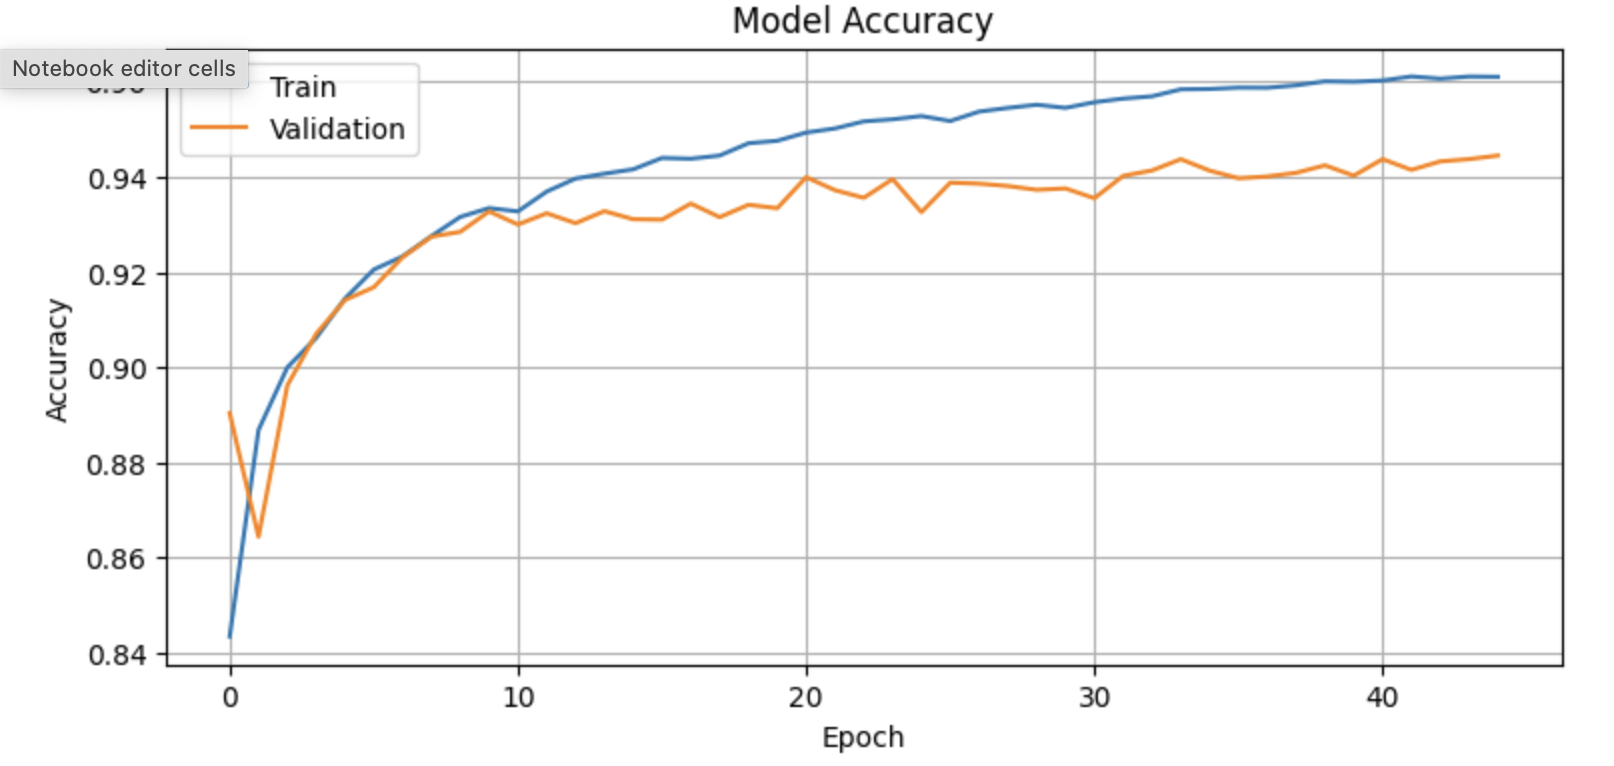
\includegraphics[width=1\textwidth]{figs/Accuracy.png}
    \caption{Accuracy Curve}
    \label{accuracy}
\end{figure}

\\

\begin{figure}[H]
    \centering
    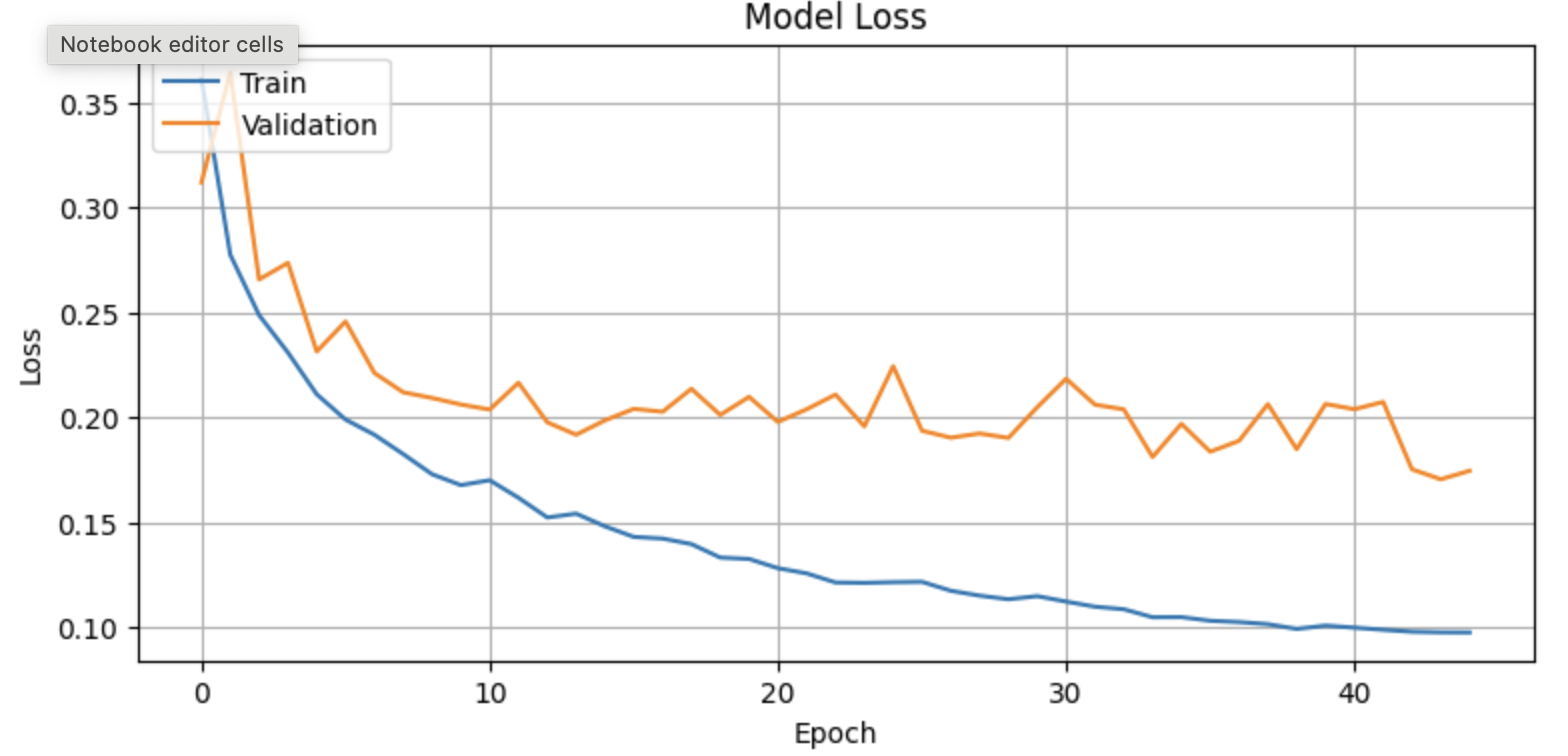
\includegraphics[width=1\textwidth]{figs/Loss.png}
    \caption{Loss Curve}
    \label{loss}
\end{figure}

\begin{figure}[H]
    \centering
    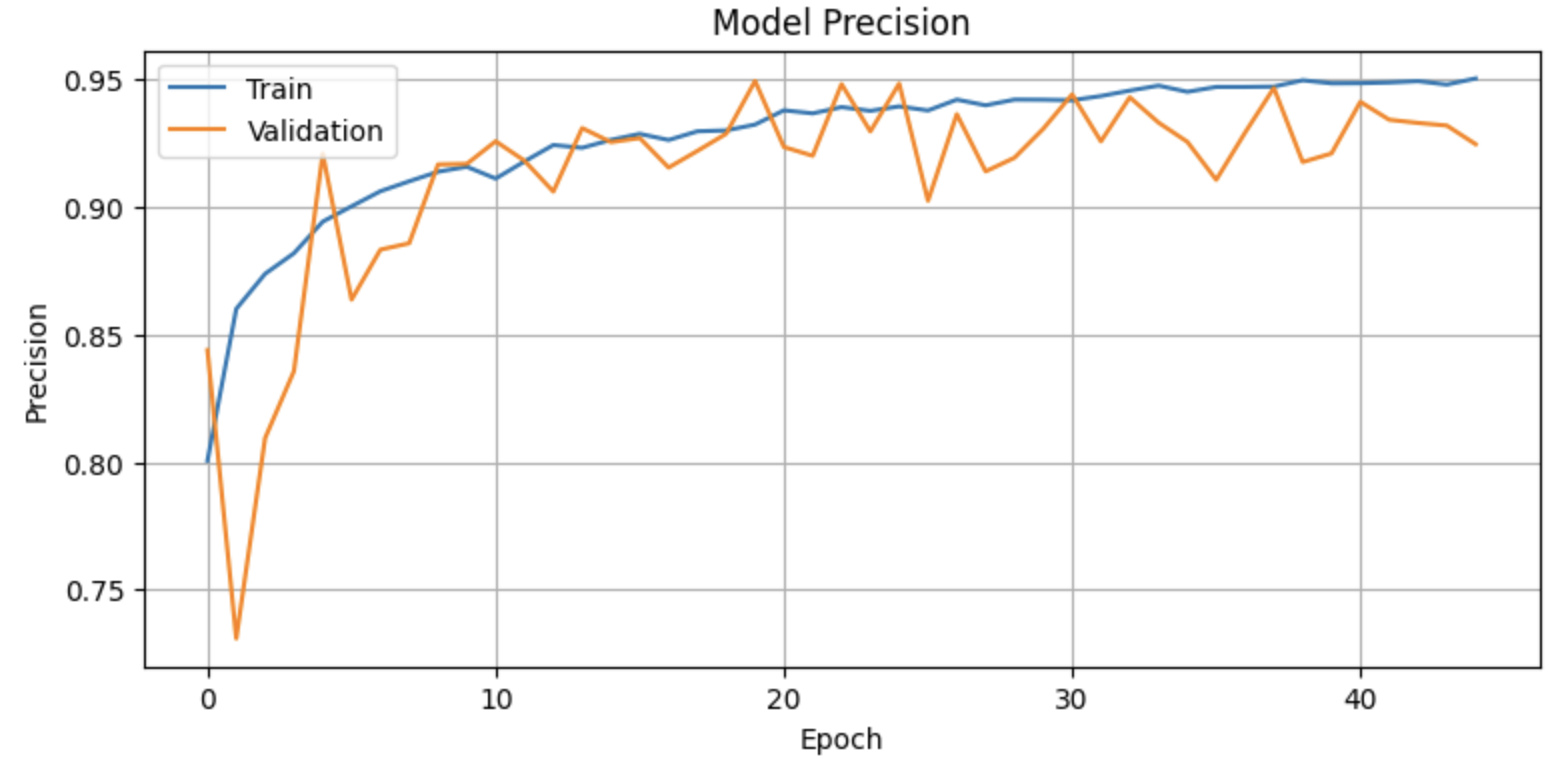
\includegraphics[width=1\textwidth]{figs/Precision.png}
    \caption{Precision Curve}
    \label{precision}
\end{figure}

\begin{figure}[H]
    \centering
    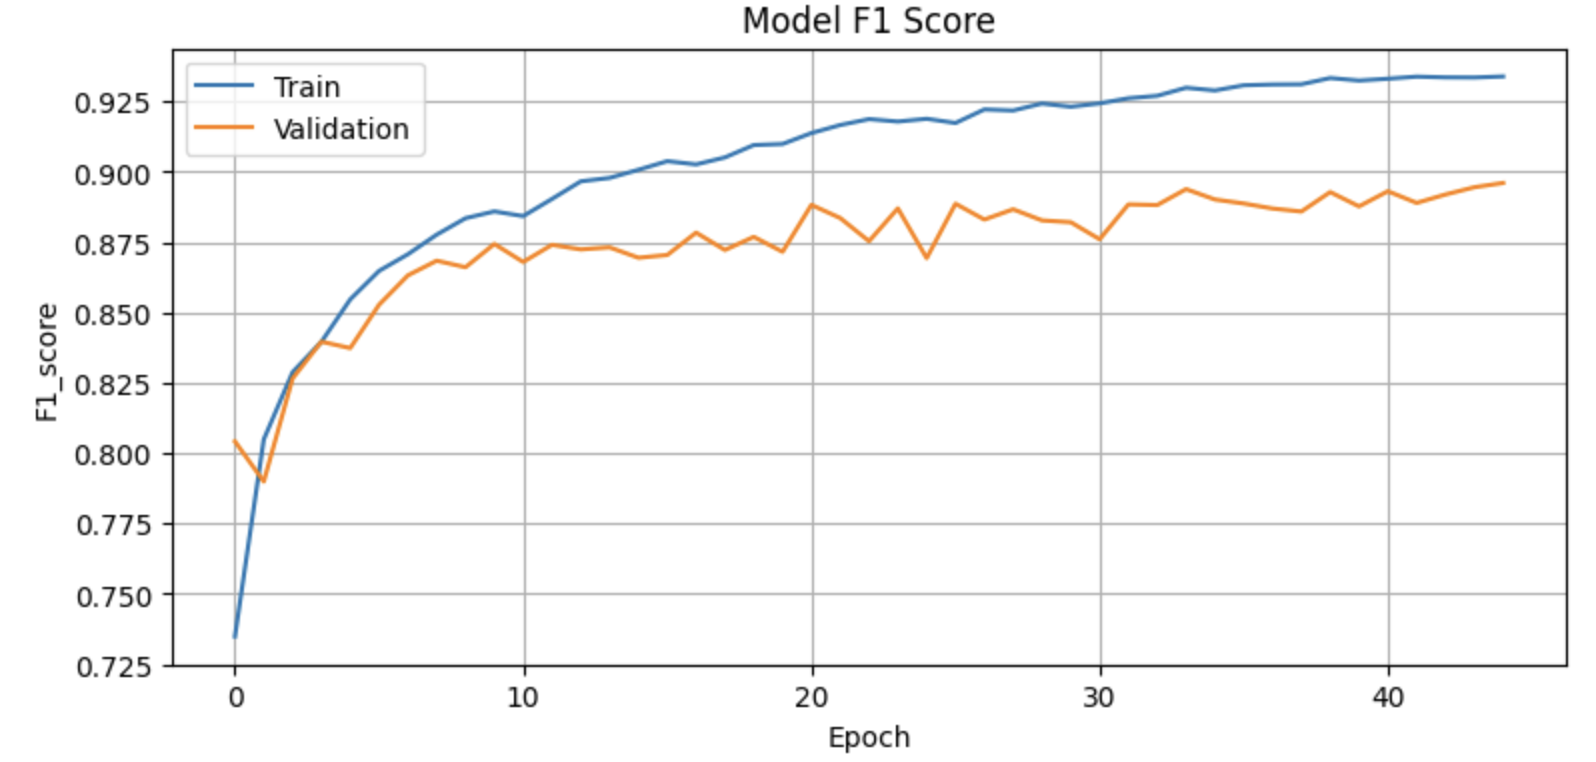
\includegraphics[width=1\textwidth]{figs/F-1 Score.png}
    \caption{F-1 Score Curve}
    \label{F-1}
\end{figure}


\begin{figure}[H]
    \centering
    \includegraphics[width=1\textwidth]{figs/IoU.png}
    \caption{mIoU Curve}
    \label{iou}
\end{figure}






\subsection{Performance Evaluation in Relation to Previous Literature}

Different research work was mentioned in the literature review.
% Among all of them \cite{res1},\cite{res2},\cite{res3} and \cite{res4} used the dataset that we did in our thesis and perform binary segmentation on the dataset.
Table 4.8 shows the different scenario among all of the works with our
proposed methods.From the table we can clearly see that our model performed better in the segmentation scenario. \\

\begin{table}[htbp]
\centering
\captionsetup{font=small} % Set font size for caption
\caption{Comparison among different existing methods and proposed method}
\label{tab:pretrained-models}
\normalsize % Set font size for table
\begin{tabular}{|p{4cm}|p{2cm}|p{1.9cm}|p{2cm}|} % Adjust column widths and add vertical lines
\hline
\textbf{Methods} & \textbf{Accuracy} & \textbf{Precision} & \textbf{Recall}\\ \hline
H.Rizk et al.\cite{per2} & 73.42\% & 73\% & 75\%\\
DP Singh et al.\cite{per3} & 76.62\% & 93.49\% & 79.44\%\\
F.Pech-may et al.\cite{per4} & 81\% & 84\% & 78\%\\
A.jamali et al.\cite{per6} & 95\% & 92\% & 69.7\%\\
T.Ahmed \cite{per5} & 80.7\% & 82\% & 79\%\\
\textbf{Proposed method} & \textbf{96\%} & \textbf{94\%} & \textbf{93\%} \\ \hline

\end{tabular}
\end{table}




\section{Impact Analysis }


The research presented in our thesis on using a weighted average ensemble model for water bodies segmentation holds significant impact across various dimensions, including scientific, practical, and environmental aspects.
From a scientific perspective, our work advances the field of semantic segmentation by demonstrating how an ensemble approach can enhance model accuracy and robustness. By integrating multiple backbones (ResNet50V2, MobileNetV3, EfficientNetV2) within the DeepLabV3+ framework, our ensemble model achieves higher segmentation accuracy compared to individual models. This advancement contributes to the existing body of knowledge on deep learning techniques, specifically highlighting the effectiveness of ensemble methods in improving performance. Additionally, the use of a weighted average method for combining predictions, based on the performance of each backbone, represents a methodological innovation that can inspire further research and application in various segmentation tasks.
Practically, our thesis provides valuable improvements in the domain of water body monitoring. The enhanced accuracy of our ensemble model facilitates better detection and mapping of water bodies, which is crucial for applications in hydrology, environmental monitoring, and land management. Accurate segmentation of water bodies supports effective water resource management by enabling precise monitoring of water levels, distribution, and changes over time. This can inform decision-making processes related to water conservation, flood management, and ecological preservation.
Environmentally, the accurate segmentation of water bodies has a direct impact on ecological studies and conservation efforts. By providing reliable data on the extent and condition of water bodies, our research aids in assessing the health of aquatic ecosystems, tracking the effects of climate change, and implementing sustainable environmental practices. Overall, our thesis not only advances the technical aspects of semantic segmentation but also contributes significantly to practical and environmental applications, highlighting the broad relevance and importance of our research.

\subsection{Social Environmental Impact}
Our thesis on using a weighted average ensemble model for water bodies segmentation carries significant social and environmental implications, influencing various aspects of society and the environment.Here are a few key aspects:
\begin{enumerate}
    \item \textbf{Environmental Conservation: }The accurate segmentation of water bodies enabled by our ensemble model contributes directly to environmental conservation efforts. By providing precise data on the extent and condition of water bodies, our research supports the assessment and monitoring of aquatic ecosystems. This information is crucial for understanding ecological health, identifying areas of concern, and implementing targeted conservation strategies.
    
    \item \textbf{Climate Change Resilience: }In the face of climate change, reliable monitoring and management of water bodies are essential. Our thesis enhances the capability to monitor changes in water levels, distribution patterns, and ecosystem dynamics over time. This data is invaluable for adapting to climate variability, predicting and managing flood risks, and safeguarding communities vulnerable to water-related disasters. 
    
    \item \textbf{Resource Management and Sustainability: }Effective water resource management is critical for ensuring sustainable development. Our ensemble model improves the accuracy of water body segmentation, thereby supporting informed decision-making in water allocation, agricultural practices, and industrial operations. This contributes to optimizing resource use, minimizing water wastage, and promoting sustainable development practices that balance environmental conservation with socio-economic needs.
    
    \item \textbf{Public Awareness and Education: }By demonstrating the application of advanced segmentation techniques in environmental monitoring, our thesis raises public awareness about the importance of water conservation and ecosystem health. It underscores the role of technology in addressing environmental challenges and encourages stakeholders to actively participate in conservation efforts.
    
    \item \textbf{Policy and Governance: }The insights and data generated from our research can inform policy development and governance frameworks related to water management and environmental protection. Our findings provide evidence-based recommendations for policy-makers, empowering them to enact legislation and regulations that prioritize environmental sustainability, protect water resources, and promote ecosystem resilience.
   
\end{enumerate}

\subsection{Economic impact}
The economic impact of this research on water bodies segmentation is substantial. Here are a few key points:

\begin{enumerate}
    \item \textbf{Optimized Resource Allocation: }Accurate segmentation of water bodies facilitated by our ensemble model enhances efficiency in resource allocation. Industries reliant on water resources, such as agriculture, manufacturing, and energy production, can benefit from precise data on water availability and distribution. This enables them to optimize water use, reduce operational costs associated with water management, and mitigate risks related to water scarcity or overuse. 
    
    \item \textbf{Infrastructure Planning and Investment: }Urban and rural development planning relies heavily on accurate environmental data, including information on water bodies. Our thesis provides reliable insights into the spatial distribution and characteristics of water bodies, aiding in infrastructure planning and investment decisions. Governments and private developers can use this information to strategically allocate resources for water infrastructure projects, such as reservoirs, dams, and drainage systems.
    
    \item \textbf{Environmental Impact Assessment (EIA) and Compliance: }n many regions, regulatory frameworks require rigorous environmental impact assessments (EIAs) for development projects affecting water bodies. Our ensemble model improves the accuracy and reliability of environmental data used in EIAs, ensuring compliance with regulatory standards and minimizing potential environmental liabilities. 
    
    \item \textbf{Eco-Tourism and Recreation: }Accurate segmentation and monitoring of water bodies support eco-tourism and recreational activities that contribute to local economies. Tourist destinations centered around lakes, rivers, and coastal areas benefit from reliable information on water quality and accessibility. Our research enhances the attractiveness of these destinations by promoting sustainable management practices and preserving natural landscapes.
    
    \item \textbf{Innovation and Technological Advancement: }The application of advanced segmentation techniques in environmental monitoring demonstrates technological innovation and fosters growth in the technology sector. Our thesis showcases the capabilities of deep learning models in addressing complex environmental challenges, stimulating research and development in artificial intelligence (AI) and machine learning (ML) applications for environmental sciences. 
    
\end{enumerate}

\subsection{Ethical Impact}
The ethical impact of this research is significant
and raises important considerations. Here are a few key points:

\begin{enumerate}
    \item \textbf{Environmental Justice and Equity: }Accurate segmentation of water bodies through our ensemble model contributes to environmental justice by ensuring fair access to clean and sustainable water resources for all communities. By providing precise data on water distribution and quality, our research supports efforts to address disparities in water access and mitigate environmental burdens disproportionately borne by marginalized or vulnerable populations.
    
    \item \textbf{Ecosystem Preservation and Conservation Ethics: }The segmentation and monitoring of water bodies facilitated by our research uphold principles of ecosystem preservation and conservation ethics. By accurately delineating water bodies and monitoring their health, our model aids in safeguarding biodiversity, protecting fragile ecosystems, and preserving natural habitats.
    
    \item \textbf{Ethical Use of Technology and Data Privacy: }As we leverage advanced segmentation techniques and AI-driven models, ethical considerations regarding technology use and data privacy become paramount. Our thesis emphasizes ethical practices in data collection, processing, and storage to protect individual privacy rights and prevent misuse of sensitive environmental data.
    
    \item \textbf{Community Engagement and Empowerment: }Engaging communities in environmental monitoring and decision-making processes is essential to ethical practice. Our research encourages community empowerment through participatory approaches, involving stakeholders in data collection, interpretation, and implementation of conservation measures. By fostering collaboration and inclusivity, our thesis promotes ethical principles of environmental governance, where communities have a voice in shaping policies and practices that affect their environment and well-being.
    
    \item \textbf{Transparency and Accountability in Environmental Management: }Our thesis promotes transparency and accountability in environmental management practices by providing stakeholders with reliable information on water resources. Transparent data-driven decisions, facilitated by accurate segmentation, enhance public trust in regulatory processes, project planning, and resource allocation.
    
\end{enumerate}



\pagebreak


\section{Conclusion}

In this chapter, we dive into the details of the data set used in our work. We
then proceed to emphasize the impact our thesis has on various aspects of society,
including the social, environmental, and ethical spheres. Finally, we provide a
thorough evaluation of the entire thesis.The model showcased commendable performance across various evaluation metrics, indicating its effectiveness in accurately identifying water areas.
With an overall accuracy of 96\%, the model demonstrated robustness in delineating water regions. Precision, Recall, and F1-score metrics further corroborated the model's accuracy and reliability in water bodies segmentation tasks. Additionally, achieving an overall IoU of 88\% underscored the model's ability to accurately align predicted masks with ground truth water areas. The fine-tuning process yielded notable improvements in performance metrics, affirming the efficacy of refining the model's parameters to better suit the task at hand. 